%\chapter{Commissioning Experiments}
\chapter[\texorpdfstring{The $^\text{28}$S\lowercase{i($d$,$p$)} Measurement}{The 28Si(d,p) Measurement}]{\texorpdfstring{The $^\mathbf{28}$Si($d$,$p$) Measurement}{The 28Si(d,p) Measurement}}
\label{exp}
%HELIOS was commissioned with a series of two ($d$,$p$) reactions in inverse kinematics.  The first reaction to be measured with HELIOS was the $^{28}$Si($d$,$p$) reaction.  This chapter describes the results of that first commissioning experiment.  
 
\section{Introduction}
\label{detail}
To demonstrate the properties of the solenoidal spectrometer technique, HELIOS was commissioned with a study of the $^{28}$Si(d,p)$^{29}$Si reaction in inverse kinematics.  As the HELIOS concept was previously untested, the commissioning experiment served as a proof of principle to verify the HELIOS performance characteristics.  The results of the commissioning experiment are reported in Ref.~\cite{Lighthall_2010}; this chapter expands on the discussion of those results. % suggested by its design. %~\cite{Schiffer_1998,Schiffer_2003,Wuosmaa_2003,Wuosmaa_2007}. 
  The $d$($^{28}$Si,$p$) reaction was chosen because it has a number of advantages for this study.  The ($d$,$p$) reaction on $^{28}$Si has been measured several times over the last six decades  and the reaction mechanisms are well understood~\cite{Kuehner_1960,Mermaz_1971, El_Bedewi_1972,Piskor_1990}. The reaction has a large, positive $Q$-value of 6.249\,MeV and typical cross sections at $\theta_\textrm{cm}=0^\circ$ are of the order of 0.5--10\,mb/sr.  There are 8 states in $^{29}$Si that are strongly populated by the ($d$,$p$) reaction with excitation energies between E$_x=0$\,MeV and E$_x=7$\,MeV.  These states are separated by an average interval of 0.91\,MeV.  
Fig.~\ref{nor_kin_spec} shows a representative excitation energy spectrum for the $^{28}$Si(d,p) reaction performed in normal kinematics by \citet{Mermaz_1971}. The measurement has a reported $Q$-value resolution of 60\,keV and serves as a benchmark for comparison for transfer reactions in normal and inverse kinematics. 
  
\begin{figure*}%
\centering
%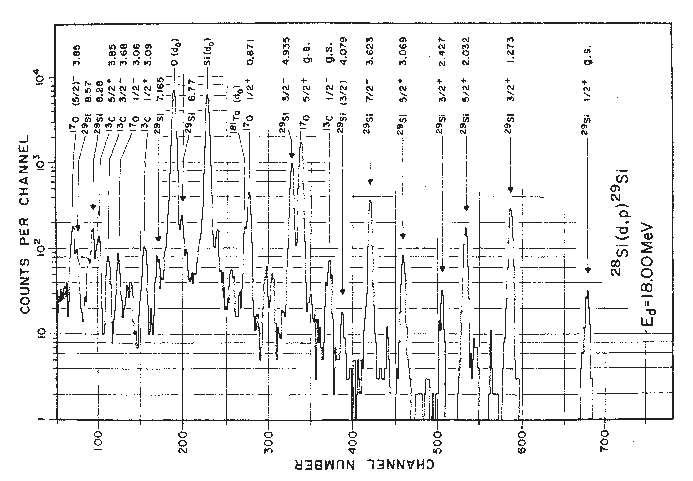
\includegraphics[width=\columnwidth,keepaspectratio]{Mermaz_1971_fig4}%
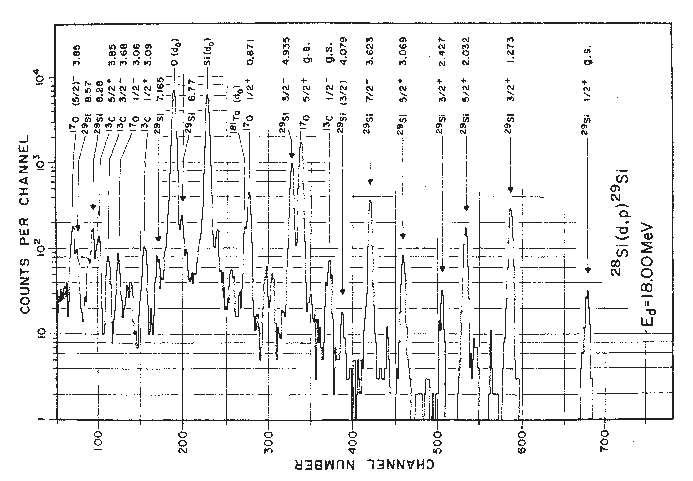
\includegraphics[height=\columnwidth,width=0.8\textheight,keepaspectratio,angle=270]{Mermaz_1971_fig4}%
\caption[Proton spectrum from the $^{28}$Si(d,p)$^{29}$Si reaction in normal kinematics]{Proton spectrum from the $^{28}$Si(d,p)$^{29}$Si reaction in normal kinematics.  The spectrum was measured measured at $\theta_\mathrm{lab}=45^\circ$, with a bombarding energy of 9.0\,\AMeV.  The peaks are labeled with the corresponding residual nucleus and the spin, parity, and excitation energy of the state populated in that nucleus.  States in $^{17}$O are populated due to the use of a silicon oxide target and states in $^{12}$C are present because of carbon contamination in the target.  States labeled with ($d_0$) are elastically scattered deuteron.  Figure from \citet[Fig.~1]{Mermaz_1971}.}%
\label{nor_kin_spec}%
\end{figure*}  
  
In $^{29}$Si there exists a pair of states near 6.2\,MeV that are separated by separated by 187\,keV.  Resolving these states in inverse kinematics is a challenge.  Table~\ref{error_prop} shows that under ideal conditions, the $Q$-value resolution of this reaction would be, at best, on the order of 116\,keV for a measurement made using a standard detection technique.  However, as stated in Ref.~\cite{Wuosmaa_2007} and shown in Table~\ref{helios_error}, the same measurement made with HELIOS should have a $Q$-value resolution on the order of the intrinsic detector resolution (neglecting beam and target effects).  Therefore, the resolution of the members of this doublet would clearly demonstrate the $Q$-value resolution achievable with this device.

\section{Experimental Setup}
The commissioning experiment was carried out using the Argonne Tandem Linear Accelerator System (ATLAS) at Argonne National Laboratory in August 2008, less than two years after the arrival of the solenoid.  A beam $^{28}$Si ions was accelerated from the ECR ion source in charge-state $+11$ to an energy of $168.52\pm0.12$\,MeV (6.024\,\AMeV{}).  The measured energy of the beam throughout the experiment is plotted in Fig.~\ref{beam_energy} (on p.~\pageref{beam_energy}). The beam was bunched with the characteristic 82\,ns packet spacing of ATLAS with a timing resolution of 0.471\,ns~FWHM. For each of the data sets presented below, the beam was incident on an 84\,$\mu$g/cm$^2$ target of deuterated polyethylene (C$_2$D$_4$)$_n$ with an average beam intensity of 25\,ppA.  This target thickness was used in order to minimize energy straggling in the target and to emphasize the resolution properties of the spectrometer.  The magnetic field of the solenoid was set to a central value of $\mathscr{B}_0=2.00$\,T.  

The leading edge of the active region of the detector array was positioned at $-$250\,mm with respect to the center of the magnet.  The detector array remained in this position throughout the course of the experiment.  To cover different center-of-mass angle ranges, the target was placed at three different positions during the experiment.  The position settings are summarized in Table~\ref{coverage_helios}. % are: 94\,mm,342\,mm, and 492\,mm away from the detector array.
For the ground-state transition in $^{28}$Si($d$,$p$), the array covered a  %center-of-mass angle %range of 37.5$^\circ$ to 52.5$^\circ$, 21.5$^\circ$ to 42.0$^\circ$, and 7.1$^\circ$ to 34.5$^\circ$, respectively.  The 
total axial  range of 743\,mm, corresponding to forward proton center-of-mass angle range of 49.4$^\circ$.

\begin{table}%
\centering
\begin{tabular}{cd{2}d{1}d{2}rrcrrcc}
Set&\multicolumn{1}{c}{Target}&\multicolumn{1}{c}{Array}&\multicolumn{1}{c}{$\Delta z$}
&\multicolumn{2}{c}{$\theta_\mathrm{lab}$}&&\multicolumn{2}{c}{$\theta_\mathrm{cm}$}&$\Delta \cos(\theta_\mathrm{cm})$&$\Delta \Omega$\\ \cline{5-6} \cline{8-9}
&\multicolumn{1}{c}{(mm)}&\multicolumn{1}{c}{(mm)}&\multicolumn{1}{c}{(mm)}&\multicolumn{1}{c}{$\theta_1$}&\multicolumn{1}{c}{$\theta_2$}&&\multicolumn{1}{c}{$\theta_1$}&\multicolumn{1}{c}{$\theta_2$}&&(sr)\\
\hline \hline
I  &-155.75&-250.0& 94.25& 93.7&111.4&&52.5&37.3&0.164&0.49~(0.31)\\
II &  92.25&-250.0&342.25&105.4&135.9&&42.0&21.3&0.166&0.50~(0.31)\\
III& 241.60&-250.0&491.60&115.1&173.1&&34.5& 3.1&0.156&0.47~(0.28)\\ \cline{9-10}
 &&& \multicolumn{6}{r}{Total} &0.390&1.18~(0.72)\\
 
 \hline
\end{tabular}
\caption[Detector positions and solid angle coverage for the $^{28}$Si($d$,$p$) measurement]{Detector positions and solid angle coverage for the $^{28}$Si($d$,$p$) measurement.  The target was positioned at three different distances from the detector array during the experiment.  The total ground-state solid angle coverage of 1.18\,sr is less than the sum of the individual ranges because the detector positions overlapped.  The solid angle coverage for setting~III was reduced because the detectors in position~1 (furthest from the target) were at a distance greater than the maximum axial range of the protons from the reaction.  The figures given in parentheses are the solid angle coverage with poorly-performing detectors excluded (see \S\,\ref{effic}).	}
\label{coverage_helios}
\end{table}

\section{Results}
\subsection{Particle Identification}
\label{results}
Particle identification was achieved by measuring the flight time of the emitted particles relative to the 82\,ns~RF period of the ATLAS beam.  Following the method described in Chapt.~\ref{calib}, the timing response of each detector was corrected for position and energy dependence.  The resulting time resolution combining all silicon detectors at all energies was 9.1\,ns~FWHM, which was sufficient to isolate the reaction products of interest.  Fig.~\ref{hTOF} shows a representative time of flight spectrum from the experiment, which has two main features.  The larger peak near 32.8\,ns represents protons that intercept the detector array at the end of one cyclotron orbit.  The smaller peak in the timing spectrum near 65.6\,ns corresponds to particles with a mass-to-charge ratio of $A/q=2$ ($\alpha$ particles and deuterons), and to protons executing two cyclotron orbits.  However, in this experiment \textit{reaction} products with an $A/q=2$ are outside of the acceptance of the array.  Since the timing resolution is energy-dependent, a two-dimensional timing cut as shown in Fig.~\ref{2d_time} was used to gate the data.  Spectra gated on both flight times are shown below.

\begin{figure}
\centering
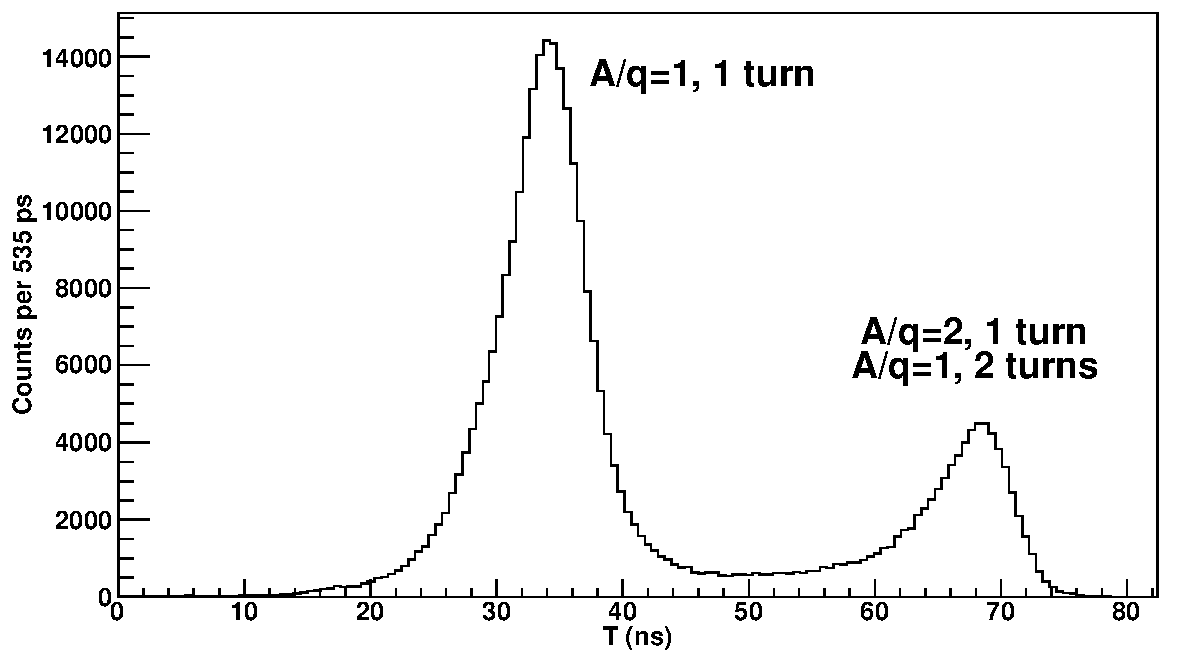
\includegraphics[width=\linewidth,]{cTOF_21_100b}
\caption[Time-of-flight spectrum for protons from $^{28}$Si+(C$_2$D$_4$)$_n$]{Time-of-flight spectrum  for protons from %emitted from
$^{28}$Si+(C$_2$D$_4$)$_n$. % collisions
 The 82\,ns accelerator RF period is covered, including all energies for an individual detector.  The peak near 33\,ns corresponds to protons completing one cyclotron orbit.  The peak at 66\,ns corresponds to protons completing two cyclotron orbits, as
well as to particles with $A/q$=2.  This figure appears similar form in Ref.~\cite{Lighthall_2010}.}
\label{hTOF}
\end{figure}

\begin{figure}
\centering
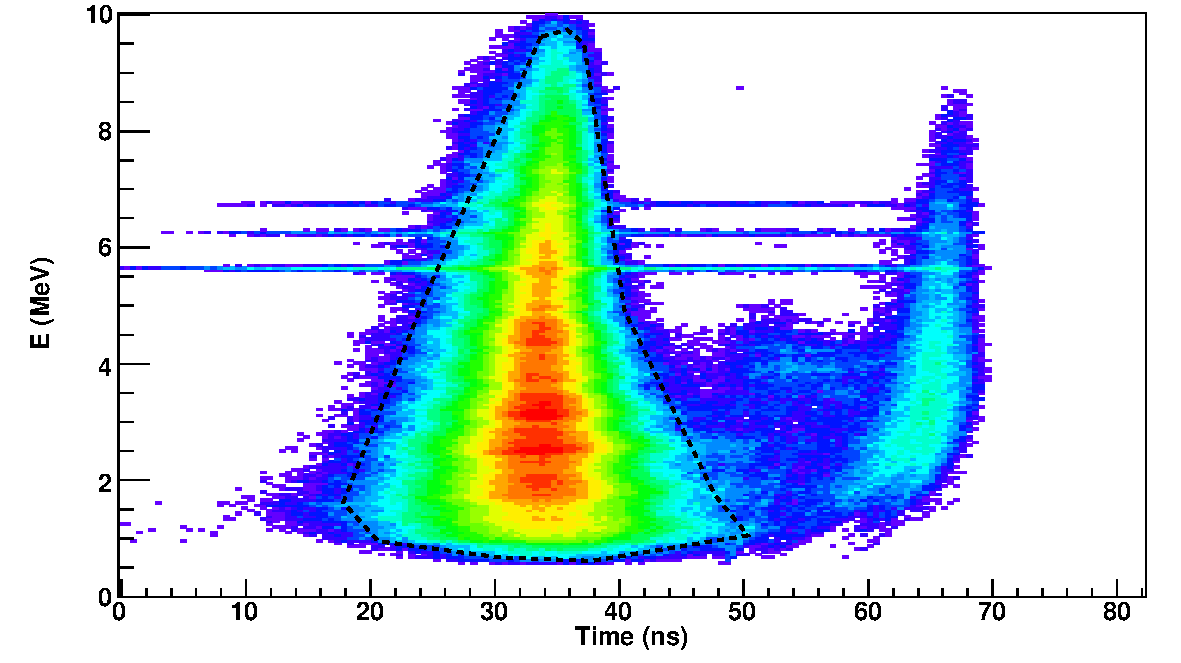
\includegraphics[width=\linewidth,keepaspectratio]{cET_big}%
\caption[Energy vs. time spectrum for all detectors at $\Delta z=94$\,mm (setting I)]{Energy vs. time spectrum for all detectors at $\Delta z=94$\,mm (setting I).  A typical two-dimensional timing gate selecting flight times corresponding to single-orbit protons has been plotted.  The bands corresponding to the $\alpha$-decay source are seen to have no time dependence (random coincidence).  The centroid of the locus near 66\,ns is energy-independent; however the low-energy time walk correction leads to the rounded cutoff starting near 3\,MeV (\textit{cf}.~Fig.~\ref{time_plot}).}%
\label{2d_time}%
\end{figure}

\subsection{Energy Resolution}
%An example of the kinematic spectrum produced in the experiment is shown in Fig.~\ref{cezg_350}.  Energy states produced in the reaction are shown as sharp, diagonal lines. 
Fig.~\ref{cezg_350} shows the measured spectrum of proton energy $E$ versus axial position $z$ for data taken with the target-to-detector separation of $\Delta z=340$\,mm (setting~II).  An energy-dependent time gate similar to the one shown in Fig.~\ref{2d_time} was used, requiring a time-of-flight consistent with single-orbit protons.    The six vertical
bands of counts correspond to the six silicon-detector positions
within the array.  The diagonal loci in the data correspond to transitions to different excited states in
the residual $^{29}$Si nucleus.  The slope of the kinematic groups is 10.1\,keV/mm (by inspection, the slope is roughly 1\,MeV/100\,mm).  The kinematic loci in the plot are overlaid with the analytically calculated position of these states and are labeled accordingly.  
The experimental data and the theoretical calculations are in excellent agreement.  The solid vertical lines indicate the outer limits to the
active region of the whole silicon-detector array.  The thick dashed
lines show the cuts in acceptance.  The transverse size of the
silicon-detector array corresponds to an acceptance limit of $\theta_\mathrm{lab} \leq 177^\circ$~(A).  
The geometry of the target frame---for target settings~II and III---produced an acceptance limit of $\theta_\mathrm{lab} \geq 113.5^\circ$~(B).  That
obstruction was corrected for data obtained at target setting I.

\begin{figure}[ht]
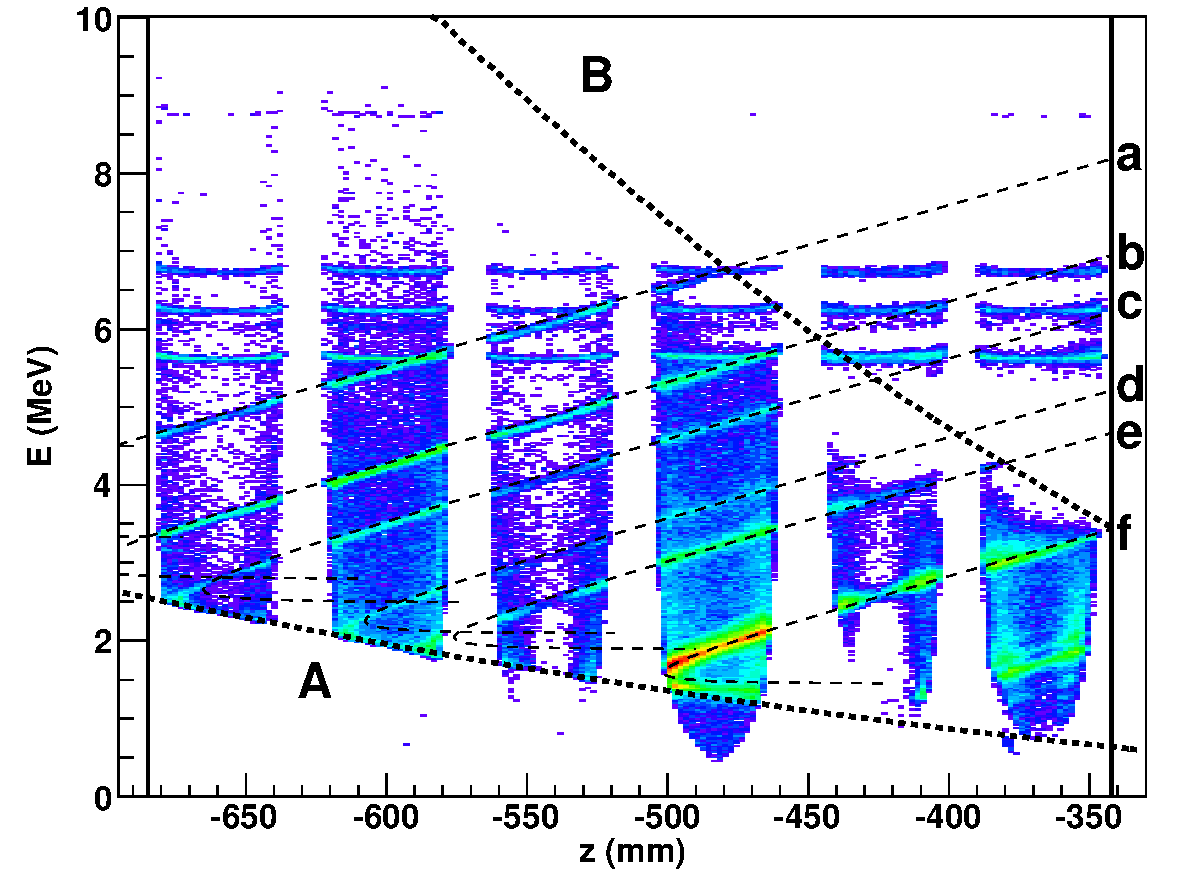
\includegraphics[width=\columnwidth]{../NIM_Paper/Figures/cEZg_350}
\caption[Energy vs. position spectrum gated on single-orbit protons at $\Delta z = 342$\,mm]{Energy vs. position spectrum gated on single-orbit protons at $\Delta z = 342$\,mm.
%Energy-versus-position spectrum 
%$\Delta z = 340$\,mm, for events with flight times consistent with
%single proton orbits.
The thin dashed lines %labeled a, b, c, d,
%e, and f
 indicate the analytically calculated position of the
kinematic groups with excitation energies of (a)~0.00, (b)~1.27, (c)~2.03, (d)~3.07,
(e)~3.62, and (f)~4.90\,MeV. %, respectively.
 The thick dashed curves are the
acceptance cutoffs discussed in the text. The pair of vertical lines
indicate the range of the array coverage for this setting.  This figure also appears in Ref.~\cite{Lighthall_2010}.}
\label{cezg_350}
\end{figure}

The backgrounds in Fig.~\ref{cezg_350} arise from two sources.  
The horizontal lines in the spectrum (fixed $E$ as a function of $z$) are correspond
to $\alpha$ particles from $^{224}$Ra contamination in the vacuum chamber from a $^{228}$Th calibration source.  The $\alpha$ particles are in random time coincidence with the accelerator RF (see Fig.~\ref{2d_time}) and cannot be
completely eliminated using a time-of-flight selection.  
Also present in the data is a smooth background of protons produced in fusion-evaporation reactions  of $^{28}$Si+$^{12}$C in the CD$_2$ target.  Protons from these reactions have the same time-of-flight as those from the reaction of
interest, and hence can also not be eliminated by a time gate alone.  In subsequent measurements, such events are distinguished using a recoil detector to detect and identify the forward-moving heavy recoils~\cite{Schiffer_2010,Wuosmaa_2010}; this detector was not implemented for the $^{29}$Si measurement.    

Only a small fraction of protons can execute two cyclotron orbits without first hitting the silicon array.  Fig.~\ref{double} shows the energy versus position spectrum at the furthest position, $\Delta z=492$\,mm (setting III), gated on a time-of-flight consistent with 65.6\,ns.  Despite
the lower statistics, diagonal loci are still present with a slope
that is half that of the single-turn data, 5.1\,keV/mm, representing transitions to
states in $^{29}$Si.  Although the acceptance for such events is
limited, as Fig.~\ref{double} shows, it is possible to extend the center-of-mass angle range
through the use of multi-turn orbits in certain situations.
The acceptance limits plotted in the figure are the same as those in Fig~\ref{cezg_350}; however, the lines are stretched in $z$ by a factor of 2 %appear at a different location 
for double orbits because of the longer flight time.

\begin{figure}[ht]
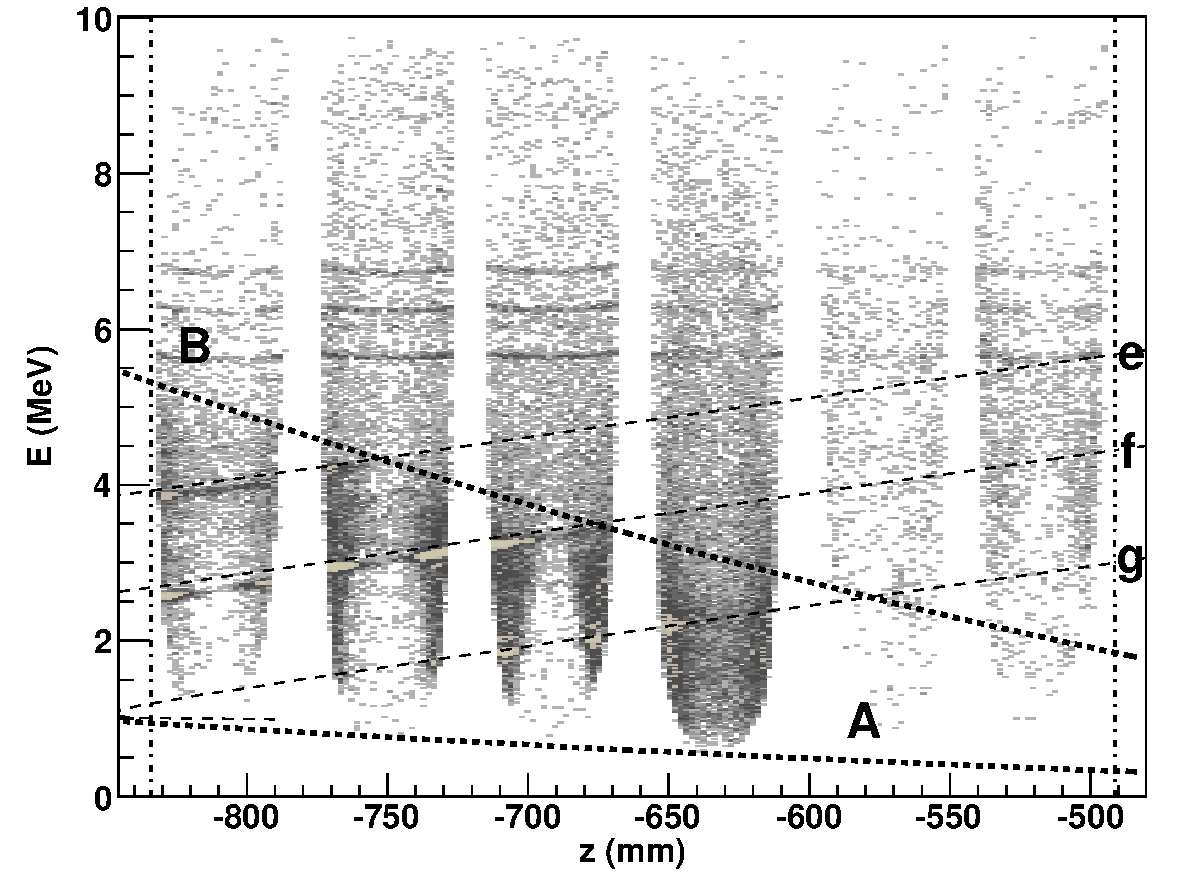
\includegraphics[width=\columnwidth]{Figures/cDouble_bw}%
\caption[Energy vs. position spectrum gated on double-orbit protons  at $\Delta z=492$\,mm]{Energy vs. position spectrum gated on double-orbit protons at $\Delta z=492$\,mm.   The thin dashed lines represent the analytically calculated energy-position
correlations for kinematic groups with excitation energies of (e)~3.62\,MeV,
(f)~4.90\,MeV, and (g)~6.38\,MeV (same labeling as Fig~\ref{cezg_350}).  The pair of vertical lines indicate the length of the array coverage.  The bold dashed lines indicate the acceptance limits of the detector array for double-orbit protons.  This figure appears similar form in Ref.~\cite{Lighthall_2010}.}%
\label{double}%
\end{figure}

Fig.~\ref{hEZ} shows a composite spectrum of proton energy versus the axial position for all three target positions.  The spectrum is gated on single-orbit protons.  The dashed curve (A) in Fig.~\ref{hEZ} indicates the acceptance limit imposed by the array. % and the wide-dashed line indicates the high-energy cutoff due to protons hitting the solenoid bore.  
Comparing the measured spectrum in Fig.~\ref{hEZ} to simulated (calculated) spectrum in Fig.~\ref{simulation} shows the relevant features predicted to be present in the spectrum are clearly reproduced.

% The gap in the data for proton energies greater than 4\,MeV 
%near $z=-380$ mm is produced by the obstruction of the target frame
%discussed above.

\begin{figure}[ht]
\centering
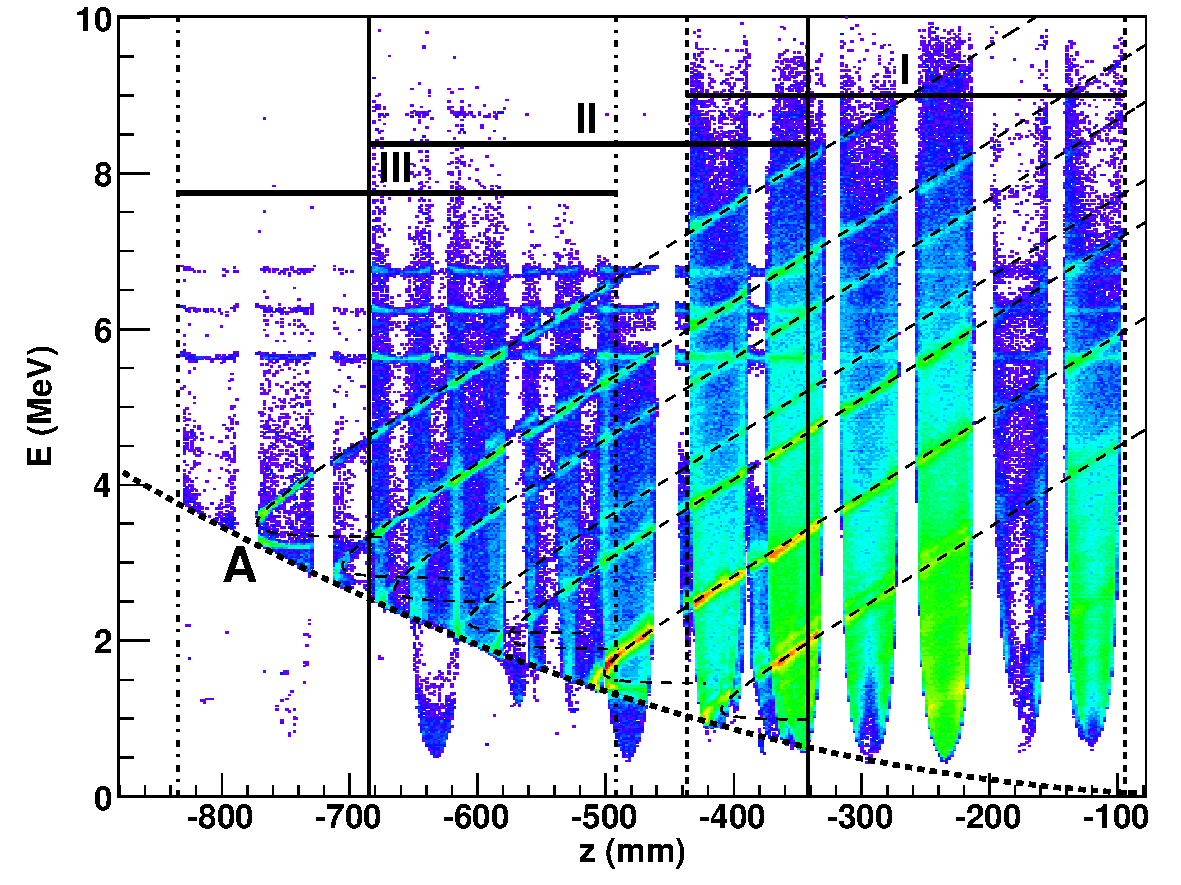
\includegraphics[width=\linewidth,keepaspectratio]{Figures/cShift}
\caption[Composite $E_\textrm{lab}$ vs. $z$ spectrum for all target positions]{Composite $E_\textrm{lab}$ vs. $z$ spectrum for all target positions.  Pairs of vertical lines indicate the length of the array coverage with leading edges at $-94$\,mm (I), $-342$\,mm (II), and $-492$\,mm (III).  The thin dashed lines are the calculated kinematic groups corresponding to excitation of 0.00, 1.27, 2.03, 3.07, 3.62, and 4.90\,MeV.  The dashed curve indicating the low-energy cutoff (A) is due to particles intercepting the front of the detector array.  This figure appears in a similar form in Ref.~\cite{Lighthall_2010}.}
\label{hEZ}
\end{figure}

Extracting the relevant center-of-mass quantities from the measured laboratory quantities is straightforward, following the prescriptions of Chapt.~\ref{HELIOS_Concept}.  The timing resolution of the HELIOS detectors in insufficient to straighten the knees in the spectrum; therefore the center-of-mass energy $E_\mathrm{cm}$ is simply obtained by projecting the laboratory energy along the slope of the kinematic loci using Eq.~\ref{ecm}.  The excitation energy is then obtained from the center-of-mass energy using Eq.~\ref{eq:recoil_mass} by accounting for the reaction $Q$-value and the recoil mass.  Fig.~\ref{qval} shows the resultant excitation energy spectra for $^{29}$Si.  A smooth background from fusion evaporation %of $^{28}$Si+$^{12}$C 
has been subtracted using the \texttt{TSpectrum} class~\cite{Morhac_2000}.  This background subtraction is shown explicitly in Fig.~\ref{qval}(c).  The $Q$-value resolution for all detectors at all positions was 127\,keV~FWHM, with the best detector having a resolution of 74\,keV~FWHM.  The measured $Q$-value resolution is within a few keV of the simulated resolution representing the \textit{ideal case} including target thickness effects (cf Table~\ref{sim_prop}).% and is on par with the intrinsic detector resolution.  
This result is an emphatic demonstration of the validity of the HELIOS concept.

\begin{figure*}[hb!]
\centering
%\includegraphics[height=0.4\textheight,width=\linewidth,keepaspectratio]{../NIM_Paper/Figures/Old_Figures/cEcX19}
%\includegraphics[height=0.4\textheight,width=\linewidth,keepaspectratio]{../NIM_Paper/Figures/Old_Figures/cExcite_all}
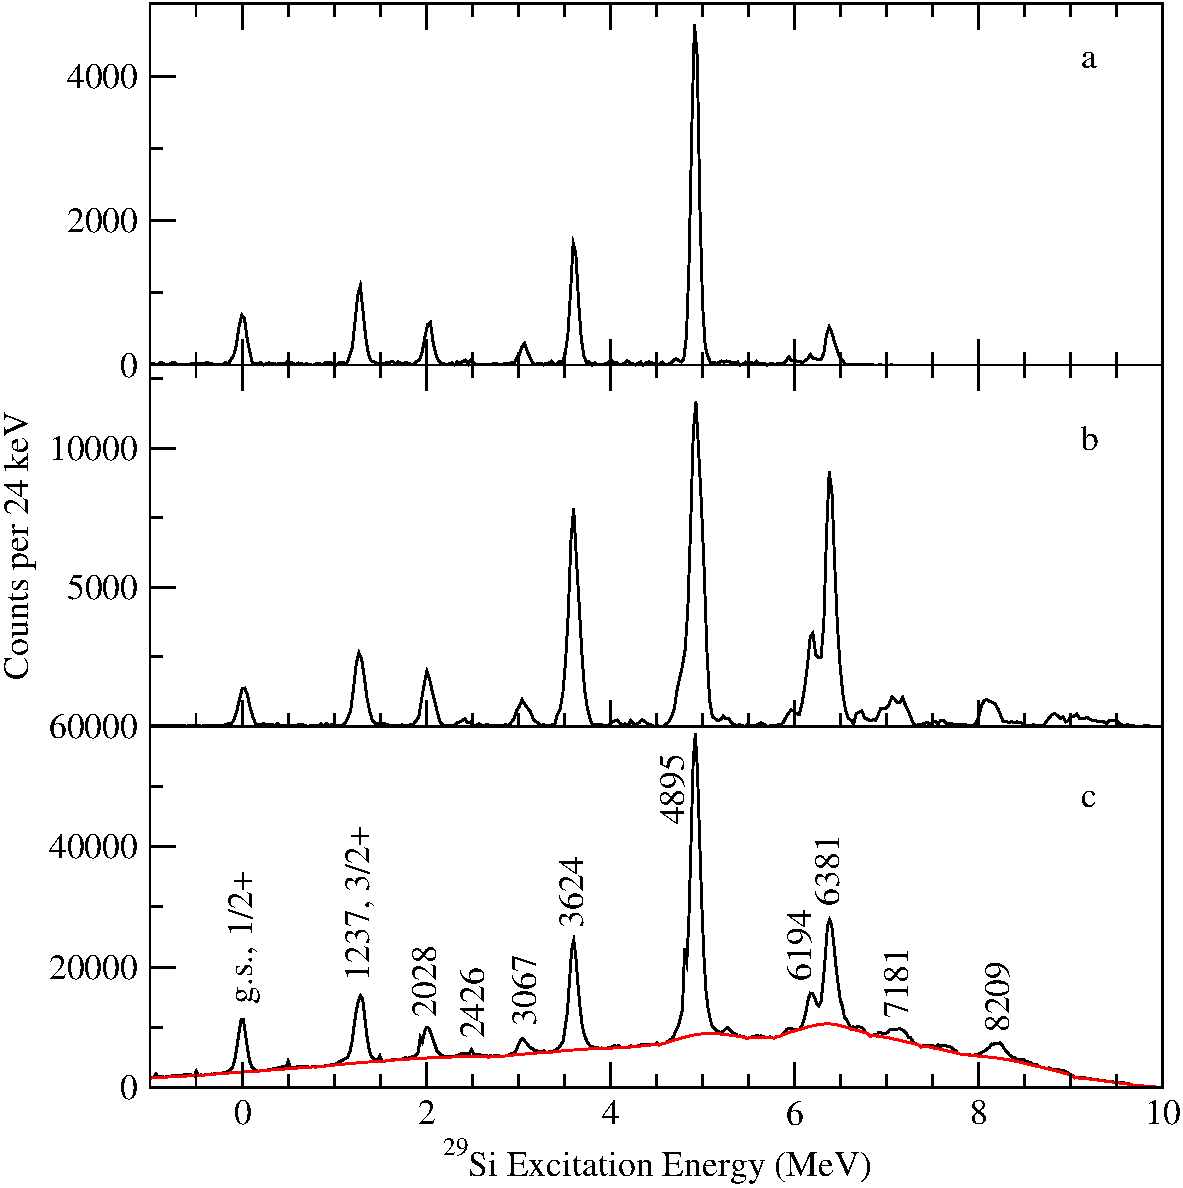
\includegraphics[width=\columnwidth]{background3}
\caption[Excitation energy spectrum for $^{29}$Si measured with HELIOS]{Excitation energy spectrum for $^{29}$Si measured with HELIOS.  
(a)~Spectrum with smooth background subtraction for an individual detector covering 386--437\,mm from the target (furthest detector position from the target with the leading edge of the array 94\,mm from the target).  The average energy resolution is 103\,keV~FWHM.  
(b)~Composite spectrum for one detector per position again with the leading edge of the array 94\,mm. 
(c)~Composite spectrum for all detectors at all three positions showing background subtraction generated by \texttt{TSpectrum}~\cite{Morhac_2000}.  The average energy resolution is 127\,keV~FWHM.  Identified energy levels are labeled by their energy in keV.  The two lowest levels are also labeled with their identified spins.  This figure appears similar form in Ref.~\cite{Lighthall_2010}.}
\label{qval}
\end{figure*}

\subsection{Efficiency}
\label{effic}
In addition to testing HELIOS as a concept, one of the goals of this commissioning experiment was to characterize HELIOS as an instrument.  Thus, not all its systems were fully optimized.  Due to a problem with signal shielding on the electronics feedthrough patch boards, 9 of the 24 detectors in the array were excluded from the trigger due to noise.  This left 2--3 active detectors at each of the six positions along the detector array, corresponding to an azimuthal coverage of 24\% or 36\%, respectively.  Additional shielding of the detector cables and patch boards 
has since eliminated this problem.  Of the remaining detectors, some can be clearly seen to have reduced efficiency towards the center of the detector. %have a significant depletion of counts in the center of the detector.

Fig.~\ref{cEZg_100} shows the energy versus position spectrum for $\Delta z = 94$\,mm (setting I) with the effect of the software energy threshold plotted as well as the regions of greatest efficiency loss.  The position- and energy-dependence of the regions of reduced efficiency is characteristic of the effect of ballistic deficit.  This is due to fact that the shaping times and electronic thresholds were not optimized for the slower rise times of the energy signals produced at these positions.  This effect is reduced by lowering the electronic threshold on the detectors, increasing the shaping time, and by including the position signals in the trigger.

\begin{figure}[th!]%
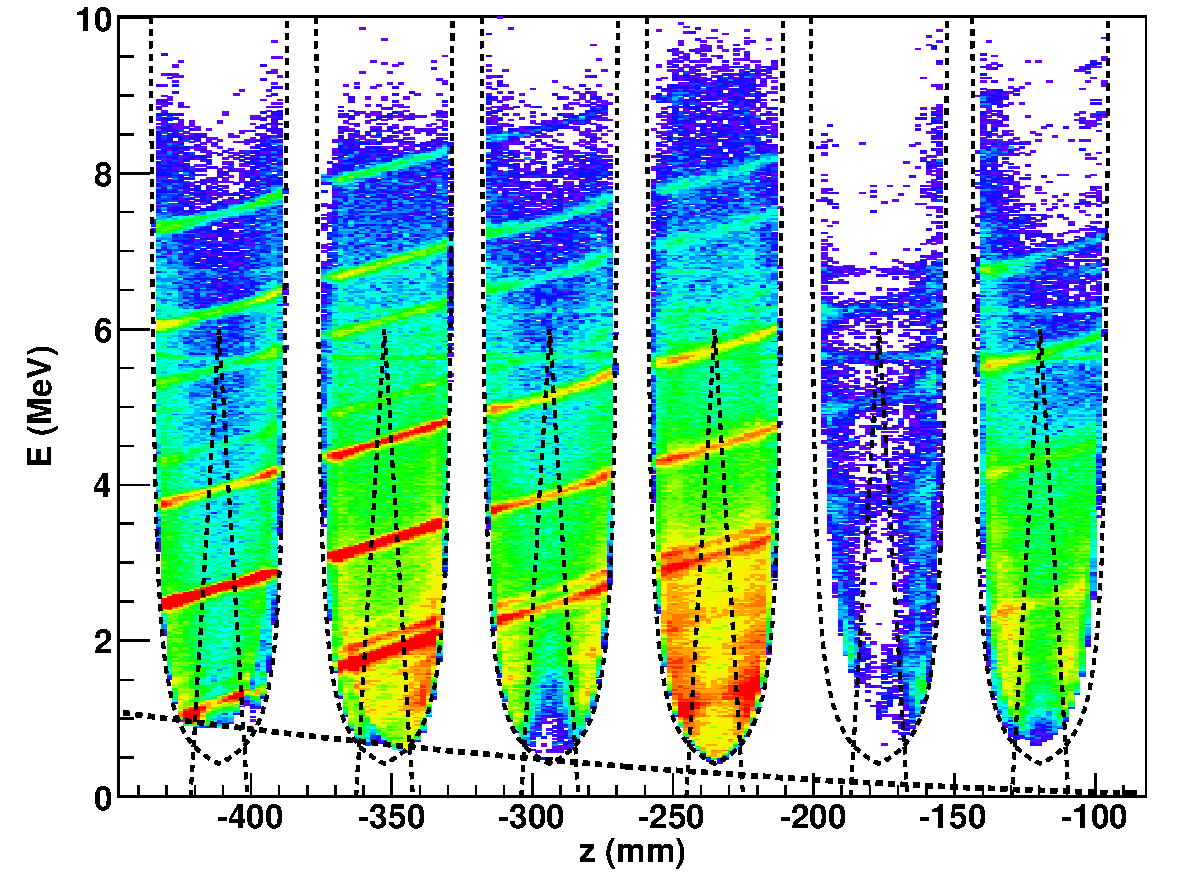
\includegraphics[width=\columnwidth]{cEZg_100_effic}%
\caption[Example of the position- and energy-dependent variations in detector efficiency]{Example of the position- and energy-dependent variations in detector efficiency.  The $E_\textrm{lab}$ vs. $z$ spectrum for $\Delta z = 94$\,mm is plotted.  The dashed U-\-shaped curves corresponds to a (software) threshold of 210\,keV required for all three signals on each detector. The dashed $\Lambda$-\-shaped curves highlight the regions where variations in energy signal rise times lead to a dramatic loss of counts.  Finally, the curve at the bottom of the figure corresponds to $\theta_\textrm{lab}=0^\circ$.}%
\label{cEZg_100}%
\end{figure}

\subsection{Angular Distributions}
The laboratory energies of the protons from the ground
and first-\-ex\-cit\-ed state transitions were sufficiently large so that the
effects of ballistic deficit were negligible.  For these states the relative detector
efficiencies were normalized to the $\alpha$ spectrum of the
$^{228}$Th calibration source. For each detector the $\alpha$ yield was used to determine the detector efficiency as a function of $X$, the detector position.  This function was then used to scale the counts for each state.  Fig.~\ref{angdist2} shows the angular distributions extracted for these two transitions using data from the
$\Delta z = 490$\,mm position setting. %for the two lowest transitions in $^{29}$Si.
Each point includes data from approximately half of one silicon detector which corresponds to a range of $\Delta \cos(\theta_\mathrm{cm})=0.014$, or $\Delta \Omega=10.6$\,msr.  The ground-state transition covers detectors 2--6 (10 points) and the first-excited state covers detectors 3--6 (8 points).  Each distribution includes one additional point 
%Center-of-mass angles
 forward of $\theta_\mathrm{cm}=10^\circ$, corresponding to the region beyond the bend of the knees where protons with
very shallow trajectories are detected well before completing their
full cyclotron orbit ($\Delta \varphi=325^\circ$%
%as discussed
); the solid-angle acceptance
for these orbits is very sensitive to the relative alignment of the
silicon array. Due to this uncertainty in the solid-angle acceptance, the forward-most data point was omitted from the ground-state angular distribution published in Ref.~\cite{Lighthall_2010}. 
 Also, in this
commissioning experiment, the beam current was not measured, and so
the cross-section scale is arbitrary.

The curves correspond to distorted-wave Born approximation calculations using the code PTOLEMY~\cite{Macfarlane_1978}.  The calculations for this reaction assume a deuteron bombarding energy of 12.09\,MeV using the optical-model parameters from listed in Table~\ref{optical_param}.  The angular distribution for the $^{29}$Si ground state shows a
shape characteristic of an angular momentum transfer of $\ell_n=0$, with
a strong maximum near $\theta_\mathrm{cm}=0^\circ$, and minimum near
$\theta_\mathrm{cm}=23^\circ$.  The transition to the ground-state is in fact an $\ell_n=0$ angular momentum transfer, corresponding to a ground-state spin assignment of $j_n=\ell_n+\frac{1}{2}=\frac{1}{2}$, with positive parity~\cite{Kuehner_1960}.  The angular distribution for the
$\frac{3}{2}^+$ first-excited state shows a much weaker dependence on
scattering angle, as expected for an $\ell_n=2$ transition.  The transition to the first excited state %at $E_x=1.27$\,MeV is an $\ell_n=2$ transfer, 
corresponding to the assignment $j_n=\ell_n-\frac{1}{2}=\frac{3}{2}$. % The patterns in Fig.~\ref{angdist} are consistent with these identifications and .
The shapes
of these angular distributions are similar to those observed by \citet{Mermaz_1971} in normal kinematics at a deuteron
bombarding energy of 18\,MeV.  The relative cross sections for the
ground- and first-excited state transitions also agree well with those
obtained by Mermaz \textit{et al.\ } which demonstrates the ability of HELIOS to provide spin assignments.

\subsection{Discussion}
\label{sidisc}
The HELIOS spectrometer was successfully commissioned by measuring the $^{28}$Si(d,p)$^{29}$Si reaction in inverse kinematics.  All of the suggested design features discussed in Ref.~\cite{Wuosmaa_2007} (summarized in Table~\ref{helios_req}) were demonstrated in this experiment.  The time resolution of 9.1\,ns was sufficient to isolate single-orbit protons from double-orbit protons.  The measurement had a large acceptance with the detector array subtending a total of 1.18\,sr over three detector array settings.  The overall $Q$-value resolution was on the order of 100\,keV~FWHM, representing a substantial improvement over ``traditional'' detector schemes (\textit{cf}. Chapt.~\ref{standards}).  A $Q$-value resolution at this level is approaching that achievable in normal kinematics where the overall resolution is dominated by the intrinsic detector resolution.  Finally, given an excitation energy and bombarding energy, the center-of-mass angles were derived to generate angular distributions.  The angular distributions provided a signature of the angular momentum transferred in the reaction and allowed for the spin assignment of the ground and first-excited states in the residual $^{29}$Si nucleus.  All of these results validate the HELIOS concept, making the commissioning experiment a resounding success.

\begin{table}[b]
\centering
\begin{tabular}{ccccccccc}
\hline
\multicolumn{2}{c}{Solenoid}  &  &
\multicolumn{3}{c}{Detectors}  & & 
\multicolumn{2}{c}{Derived}\\ \cline{1-2} \cline{4-6} \cline{8-9}
\multicolumn{1}{c}{$\mathscr{B}R$}  &  
\multicolumn{1}{c}{$\mathscr{B}L$}  & &
\multicolumn{1}{c}{$\delta z$}  &  
\multicolumn{1}{c}{$\delta E_\textrm{lab}$} &
\multicolumn{1}{c}{$\delta t$} &&
\multicolumn{1}{c}{$\Delta \Omega$}  &  
\multicolumn{1}{c}{$\delta E_\mathrm{cm}$}  \\
(T$\cdot$m)&(T$\cdot$m)&&(mm)&(keV)&(ns)&&(sr)&(keV)\\
\hline \hline
1.32&4.24&&0.85&40&9.1&&0.50&100
\\
\hline 
\end{tabular}
\caption[Nominal performance specifications of the HELIOS spectrometer]{Nominal performance specifications of the HELIOS spectrometer.  The value of $\mathscr{B}R$ and $\mathscr{B}L$ are calculated for the maximum field (2.86\,T) based on the solenoid bore (462\,mm) and the maximum range of the array ($|z|<741$\,mm), respectively. $\Delta \Omega$ is calculated for one target-to-detector setting for the $^{28}$Si($d$,$p$) reaction.  This value is a factor of two smaller than the one suggested in Table~\ref{helios_req} because of the azimuthal acceptance of the prototype array.  All other values are reported as measured.}
\label{helios_perform}
\end{table}

\pagebreak

\begin{table*}[p]
  \centering
  \begin{tabular}{ld{2}d{3}d{3}d{2}d{3}d{3}d{2}d{3}d{3}d{2}c}		
    \hline
    %\multicolumn{1}{c}{\multirow{2}{*}{%
    Particle  &  
    \multicolumn{1}{c}{$V$}  &
    \multicolumn{1}{c}{$r_0$}  &  
    \multicolumn{1}{c}{$a$}  &  
    \multicolumn{1}{c}{$W_\textrm{D}$}  &
    \multicolumn{1}{c}{$r_0^\prime$}  &  
    \multicolumn{1}{c}{$a^\prime$}  &  
    \multicolumn{1}{c}{$V_\textrm{SO}$}  &
    \multicolumn{1}{c}{$r_\textrm{SO}$}  &  
    \multicolumn{1}{c}{$a_\textrm{SO}$}  &  
    \multicolumn{1}{c}{$r_C$}  &  
     Ref. \\%\cline{2-6}
    \renewcommand{\arraystretch}{.3}
    &\multicolumn{1}{c}{(MeV)}  &\multicolumn{1}{c}{(fm)}  & \multicolumn{1}{c}{(fm)} 
    &\multicolumn{1}{c}{(MeV)}  &\multicolumn{1}{c}{(fm)}  & \multicolumn{1}{c}{(fm)} 
    &\multicolumn{1}{c}{(MeV)}  &\multicolumn{1}{c}{(fm)}  & \multicolumn{1}{c}{(fm)}  
    & \multicolumn{1}{c}{(fm)}    & \\
    \hline \hline 
		%\multicolumn{1}{c}{\multirow{1}{*}{%
		Deuteron
		% V    &  r0   &  a0   & WD     & r0`  & a0` & VSO & rSO & aSO & r0C & ref\\
		&124.7&  0.919 & 0.943 &  22.4  & 1.422&0.541
		&\multicolumn{1}{c}{---}&\multicolumn{1}{c}{---}&\multicolumn{1}{c}{---}&1.30&\cite{Mermaz_1971} \\	
		&103&    1.0   & 0.943 &  29.6  & 1.501&0.527&9.0&1.25&0.58&1.25&\cite{ElNaiem_1972} 	\\
	  &106.03& 1.051 & 0.842 &  11.24 & 1.548&0.633&7.43&0.894&0.583&1.3&\cite{Piskor_1990} \\
		%	&6.25&  8.94  &  0.04  &  180.0  & \cite{Kuehner_1960} \\
		%\multicolumn{1}{c}{\multirow{1}{*}{%
		Proton
		&44.0&   1.25  & 0.65  &  9.63  & 1.25 &0.47 &
		\multicolumn{1}{c}{---}&\multicolumn{1}{c}{---}&\multicolumn{1}{c}{---}&1.25&\cite{Mermaz_1971} \\	
		&50.31&  1.25  & 0.64  &  7.95  & 1.25 &0.74 &6.2&1.25&0.64&1.25&\cite{ElNaiem_1972} 	\\
	  &53.38&  1.170 & 0.750 &  9.02  & 1.320&0.584&6.20&1.010&0.750&1.3&\cite{Piskor_1990} \\
	 \hline
  \end{tabular}
  \caption[Optical model parameters for the $^{28}$Si($d$,$p$)$^{29}$Si reaction from various sources]{Optical model parameters for the $^{28}$Si($d$,$p$)$^{29}$Si reaction from various sources.  Ref.~\cite{Mermaz_1971} uses a parameter ($\lambda=25.0$) to scale the spin-orbit strength based on the real part of the Woods-Saxon potential $V$; hence, no additional parameters are specified.}
  \label{optical_param}
  \end{table*}

%\begin{figure}[hb]%
%\includegraphics[height=0.75\textheight,width=\columnwidth,keepaspectratio]{angdist_more_curves}%
%\caption[Angular distribution of the $^{28}$Si($d$,$p$)$^{29}$Si reaction]{Proton angular distributions for 
%transitions to the ground and first-excited states of $^{29}$Si.  The curves correspond to DWBA calculations for this reaction at a deuteron bombarding
%energy of 12\,MeV using optical-model parameters from Ref.~\cite{Mermaz_1971} (solid), Ref.~\cite{ElNaiem_1972} (dotted),  and Ref.~\cite{Piskor_1990} (dashed).}%
%\label{angdist}%
%\end{figure}

\begin{figure}[p]
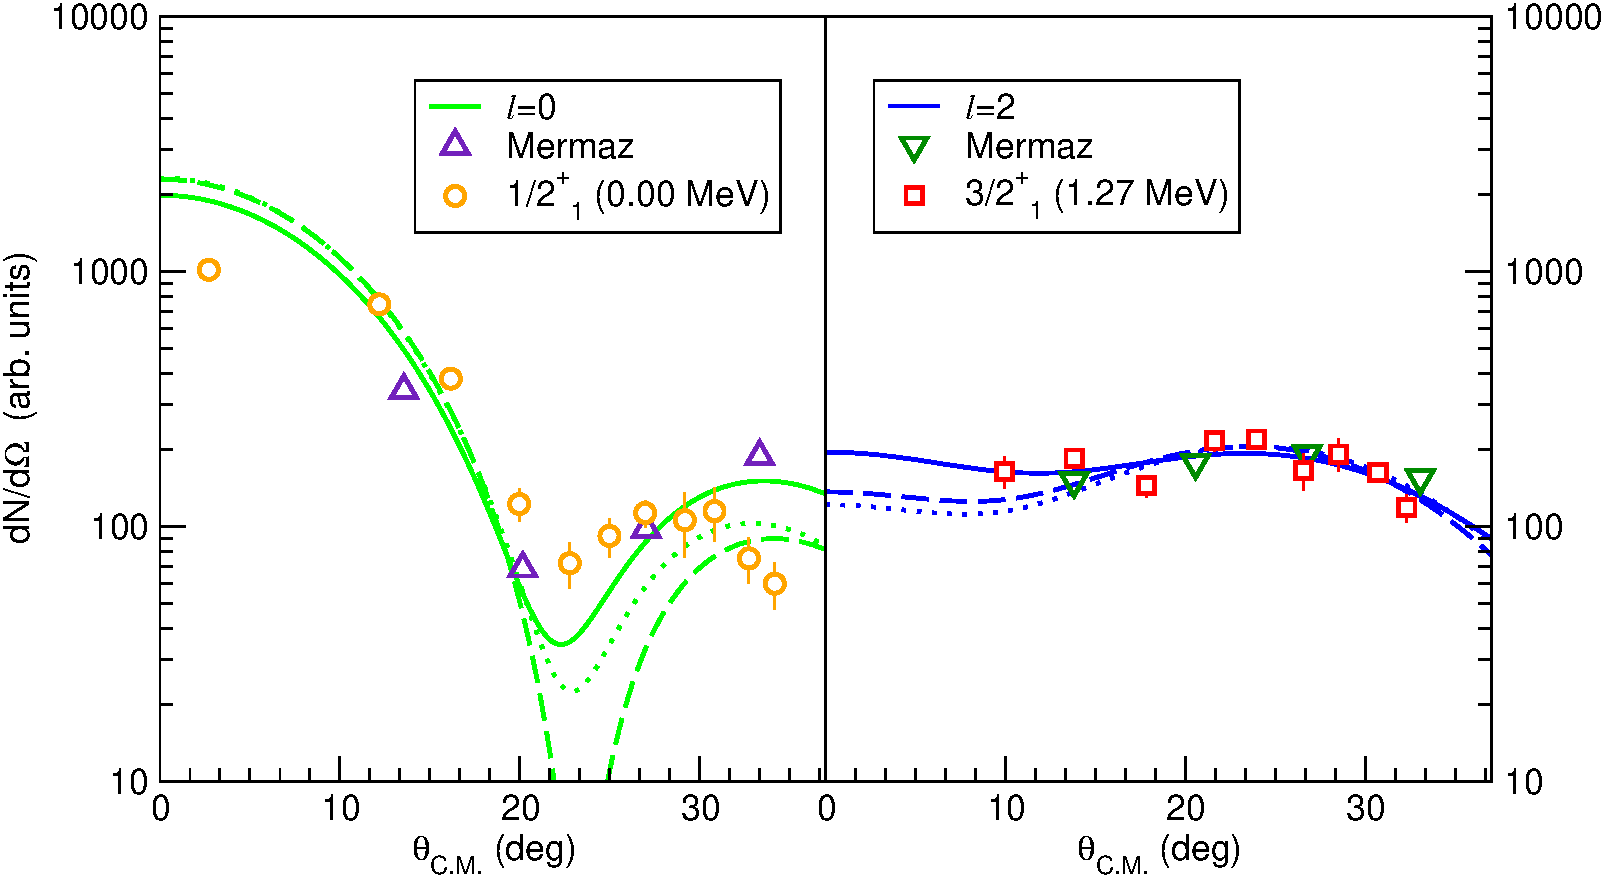
\includegraphics[height=0.75\textheight,width=0.98\columnwidth,keepaspectratio]{angdist_more_curves_comp}~
\caption[Proton angular distribution from the $^{28}$Si($d$,$p$)$^{29}$Si reaction]{Proton angular distribution from the $^{28}$Si($d$,$p$)$^{29}$Si reaction.  Transitions to the ground (left) and first-excited (right) states of $^{29}$Si are plotted.  The curves correspond to DWBA calculations for this reaction at a deuteron bombarding
energy of 12\,MeV using optical-model parameters from Ref.~\cite{Mermaz_1971} (solid), Ref.~\cite{ElNaiem_1972} (dotted),  and Ref.~\cite{Piskor_1990} (dashed).  The angular distributions from Mermaz \textit{et al.\ } have been digitized and plotted (triangles) for comparison.  The cross section of the Mermaz data have been scaled to fit the plotted DWBA calculations, and the angles in both plots have been scaled by the same factor ($\approx 23^\circ/18^\circ$, see Fig.~\ref{dwba_ediff}) to align the first minimum in the $\ell_n=0$ distribution.}%
\label{angdist2}%
\end{figure}

